\documentclass[12pt]{article}
\usepackage[margin=1.0in]{geometry}
\usepackage{graphicx}
\bibliographystyle{plain}
\usepackage{mathtools}
\usepackage{subfigure}

\begin{document}

\section{Specific Aim 2.1}

SET domain protein models of SETD2, NSD1, and NSD2 were built using Modeller with PDBs 4FMU, 3OOI, and 3OOI as inputs, respectively.  Proteins were placed in TIP3P water boxes of approximately 7 nm, with NaCl ions added to achieve neutrality.  The ff99sb-ildn force field \cite{} was used.  Systems were held at constant temperature (300K) and pressure (1 atmosphere) using a Langevin integrator and Monte Carlo barostat, as implemented in OpenMM 6.0.1 \cite{}.  For each system, a total of 10-20 $\mu s$ of simulations was analyzed using MDTraj, MSMBuilder \cite{}, and Mixtape \cite{}.  Slow coordinates were selected using temporal independent component analysis (TICA) \cite{} with randomly selected distances as inputs.  Five-state Gaussian Hidden Markov Models were constructed in the basis of the two slowest linear combinations of features.

\begin{figure}
\subfigure[]{
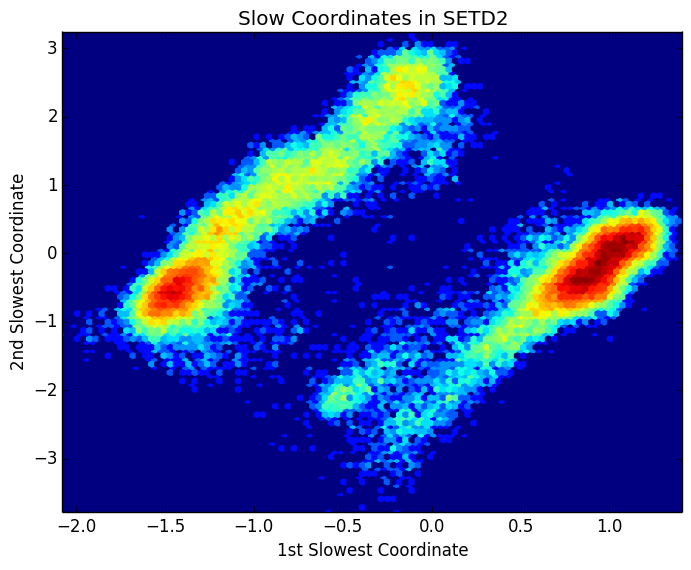
\includegraphics[width=5.0cm]{figures/SETD2_tics.png}
}
\subfigure[]{
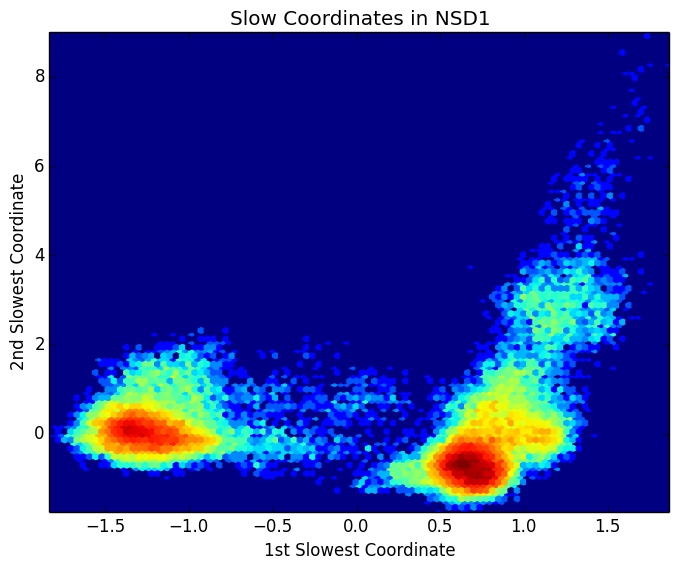
\includegraphics[width=5.0cm]{figures/NSD1_tics.png}
}
\subfigure[]{
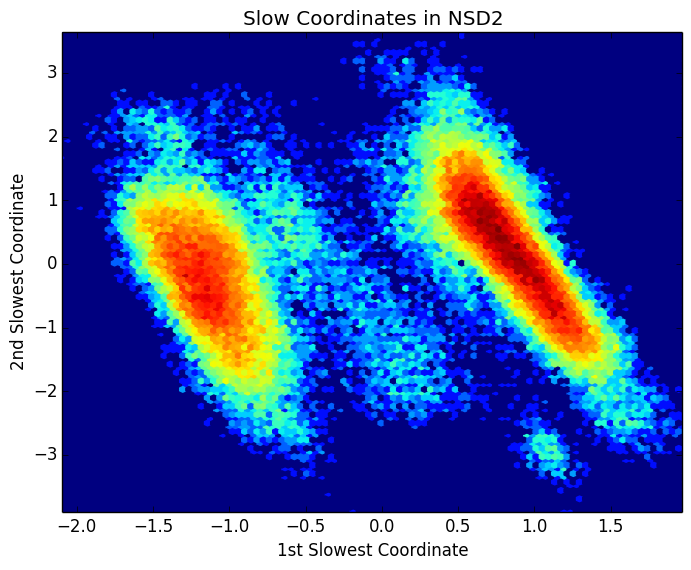
\includegraphics[width=5.0cm]{figures/NSD2_tics.png}
}


\subfigure[]{
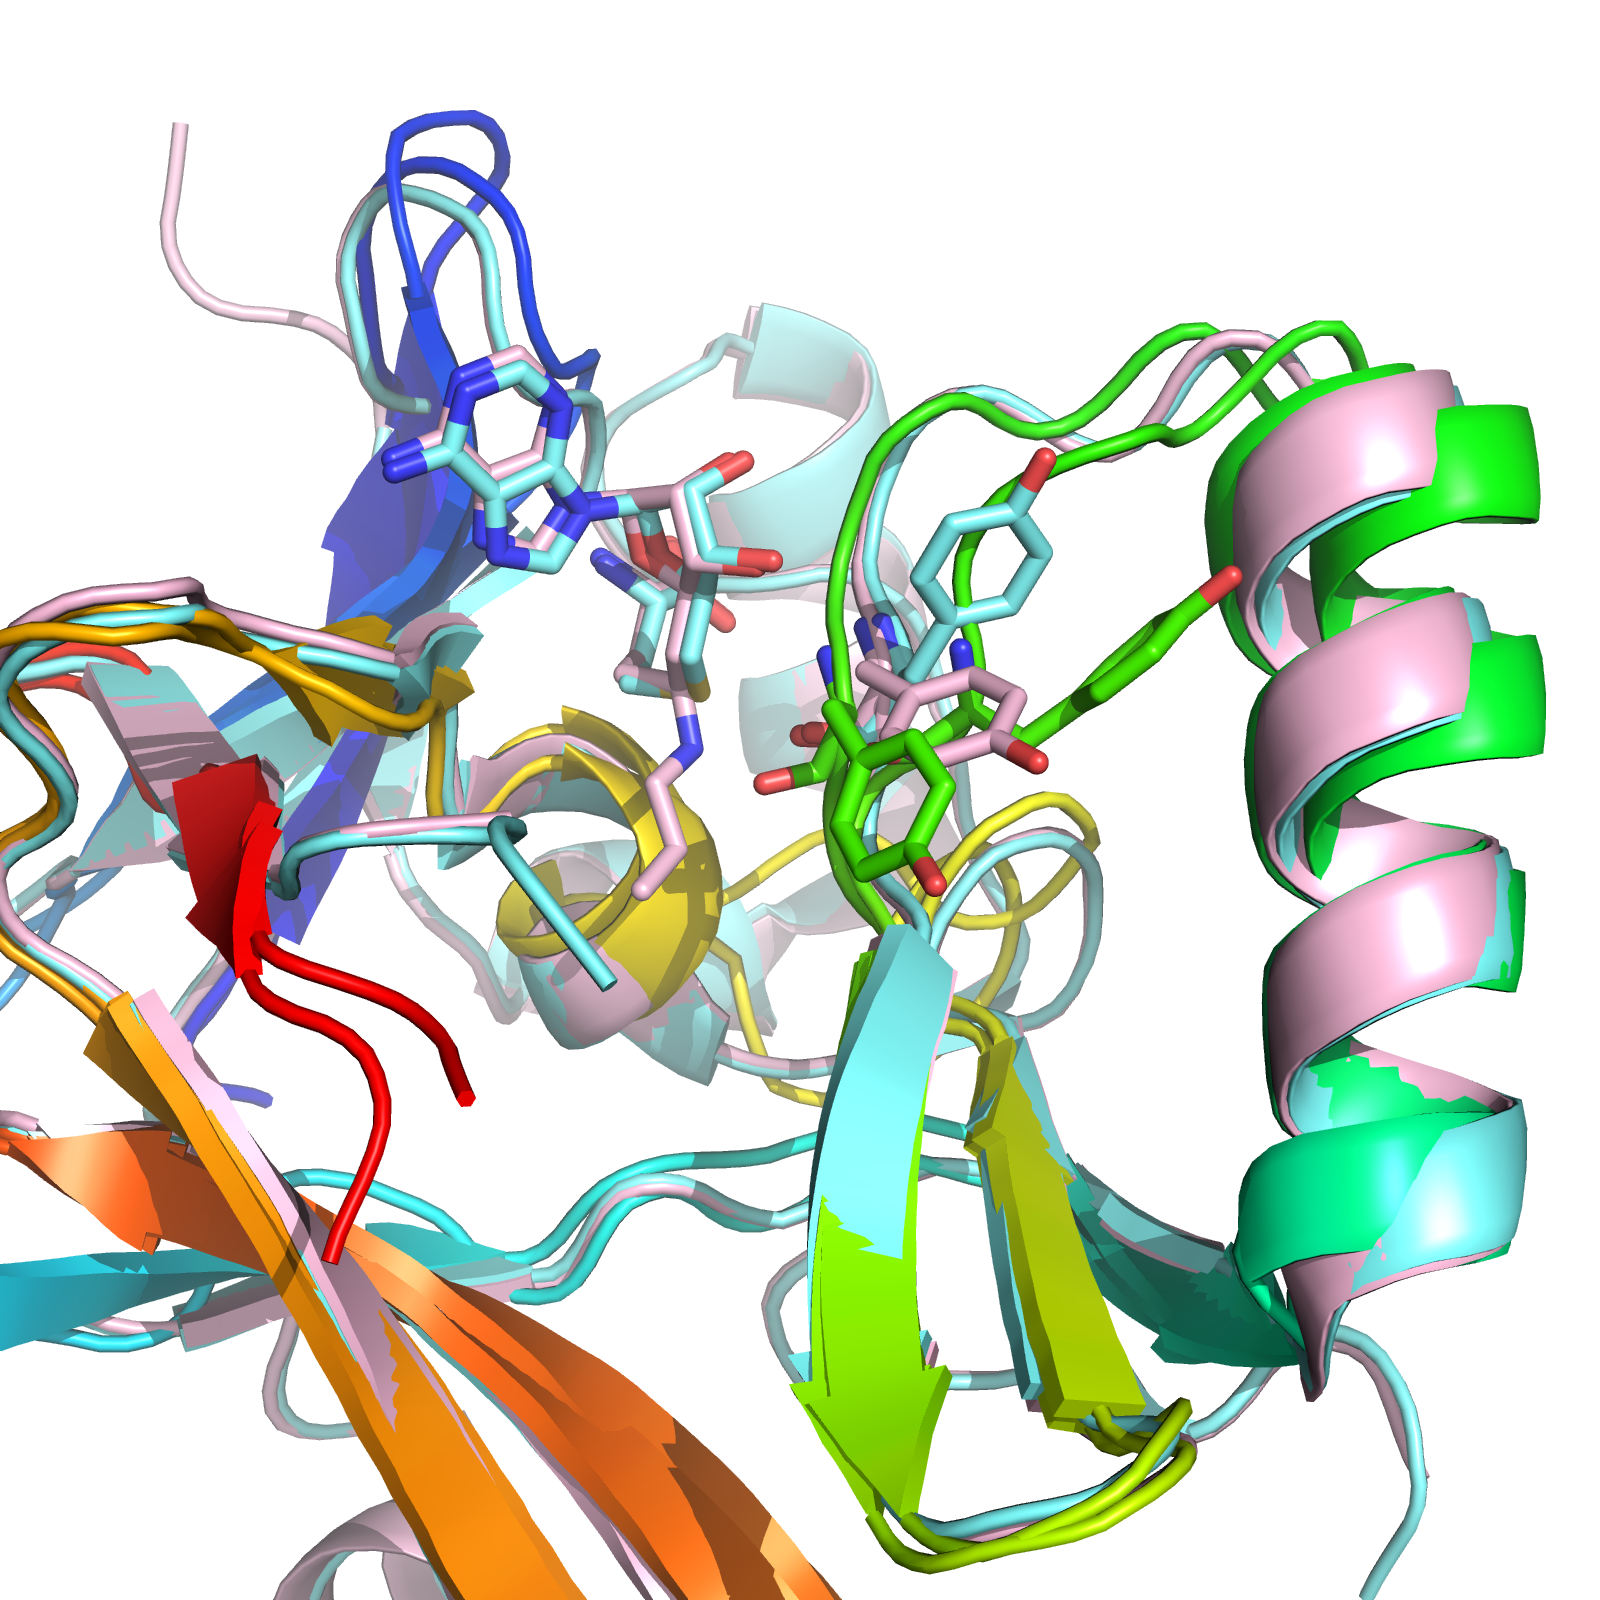
\includegraphics[width=5.0cm]{figures/SETD2_pdb.png}
}
\subfigure[]{
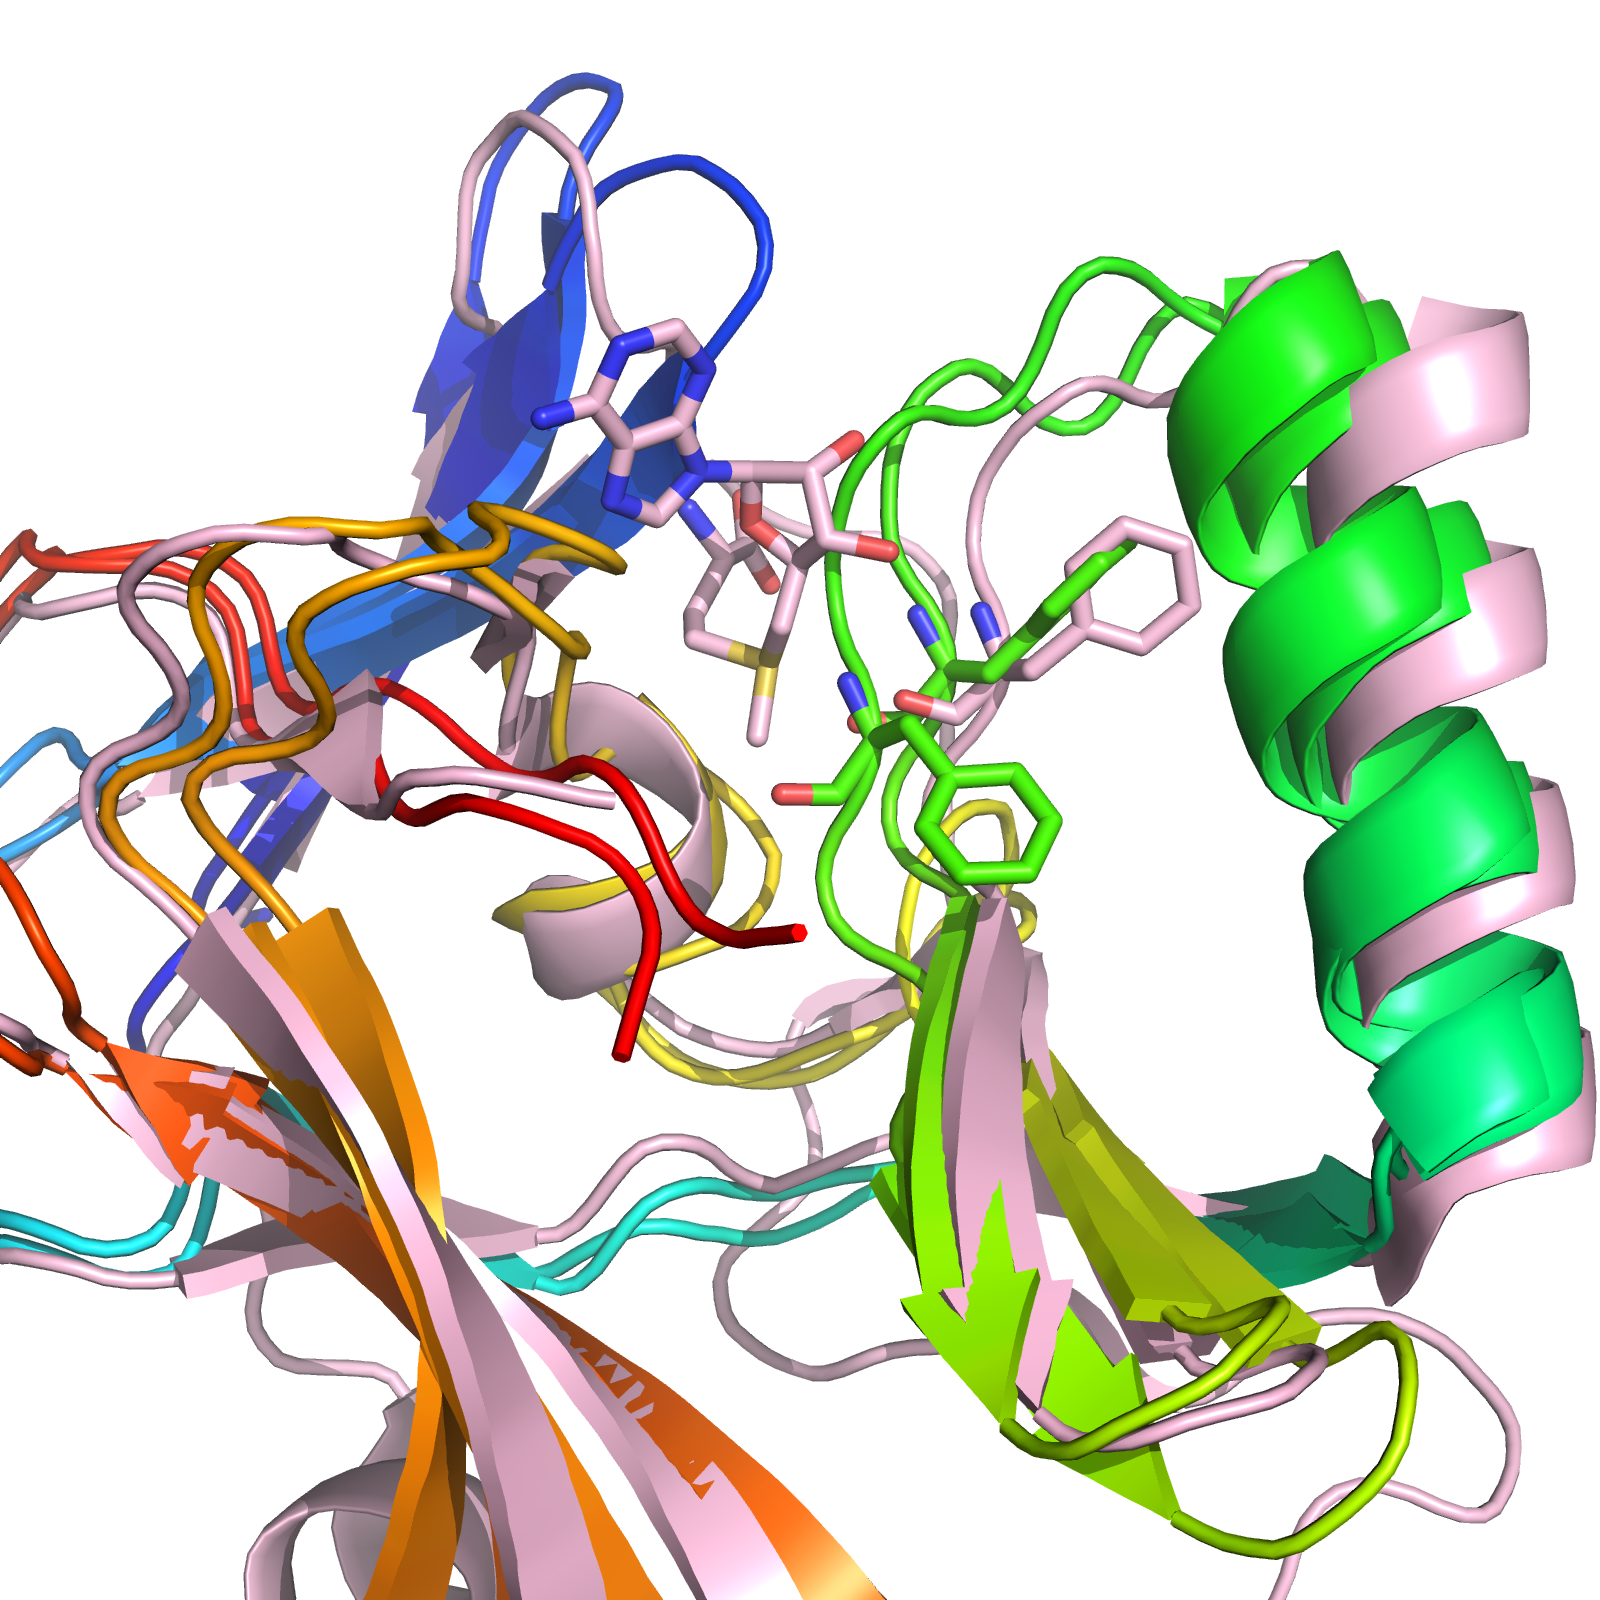
\includegraphics[width=5.0cm]{figures/NSD1_pdb.png}
}
\subfigure[]{
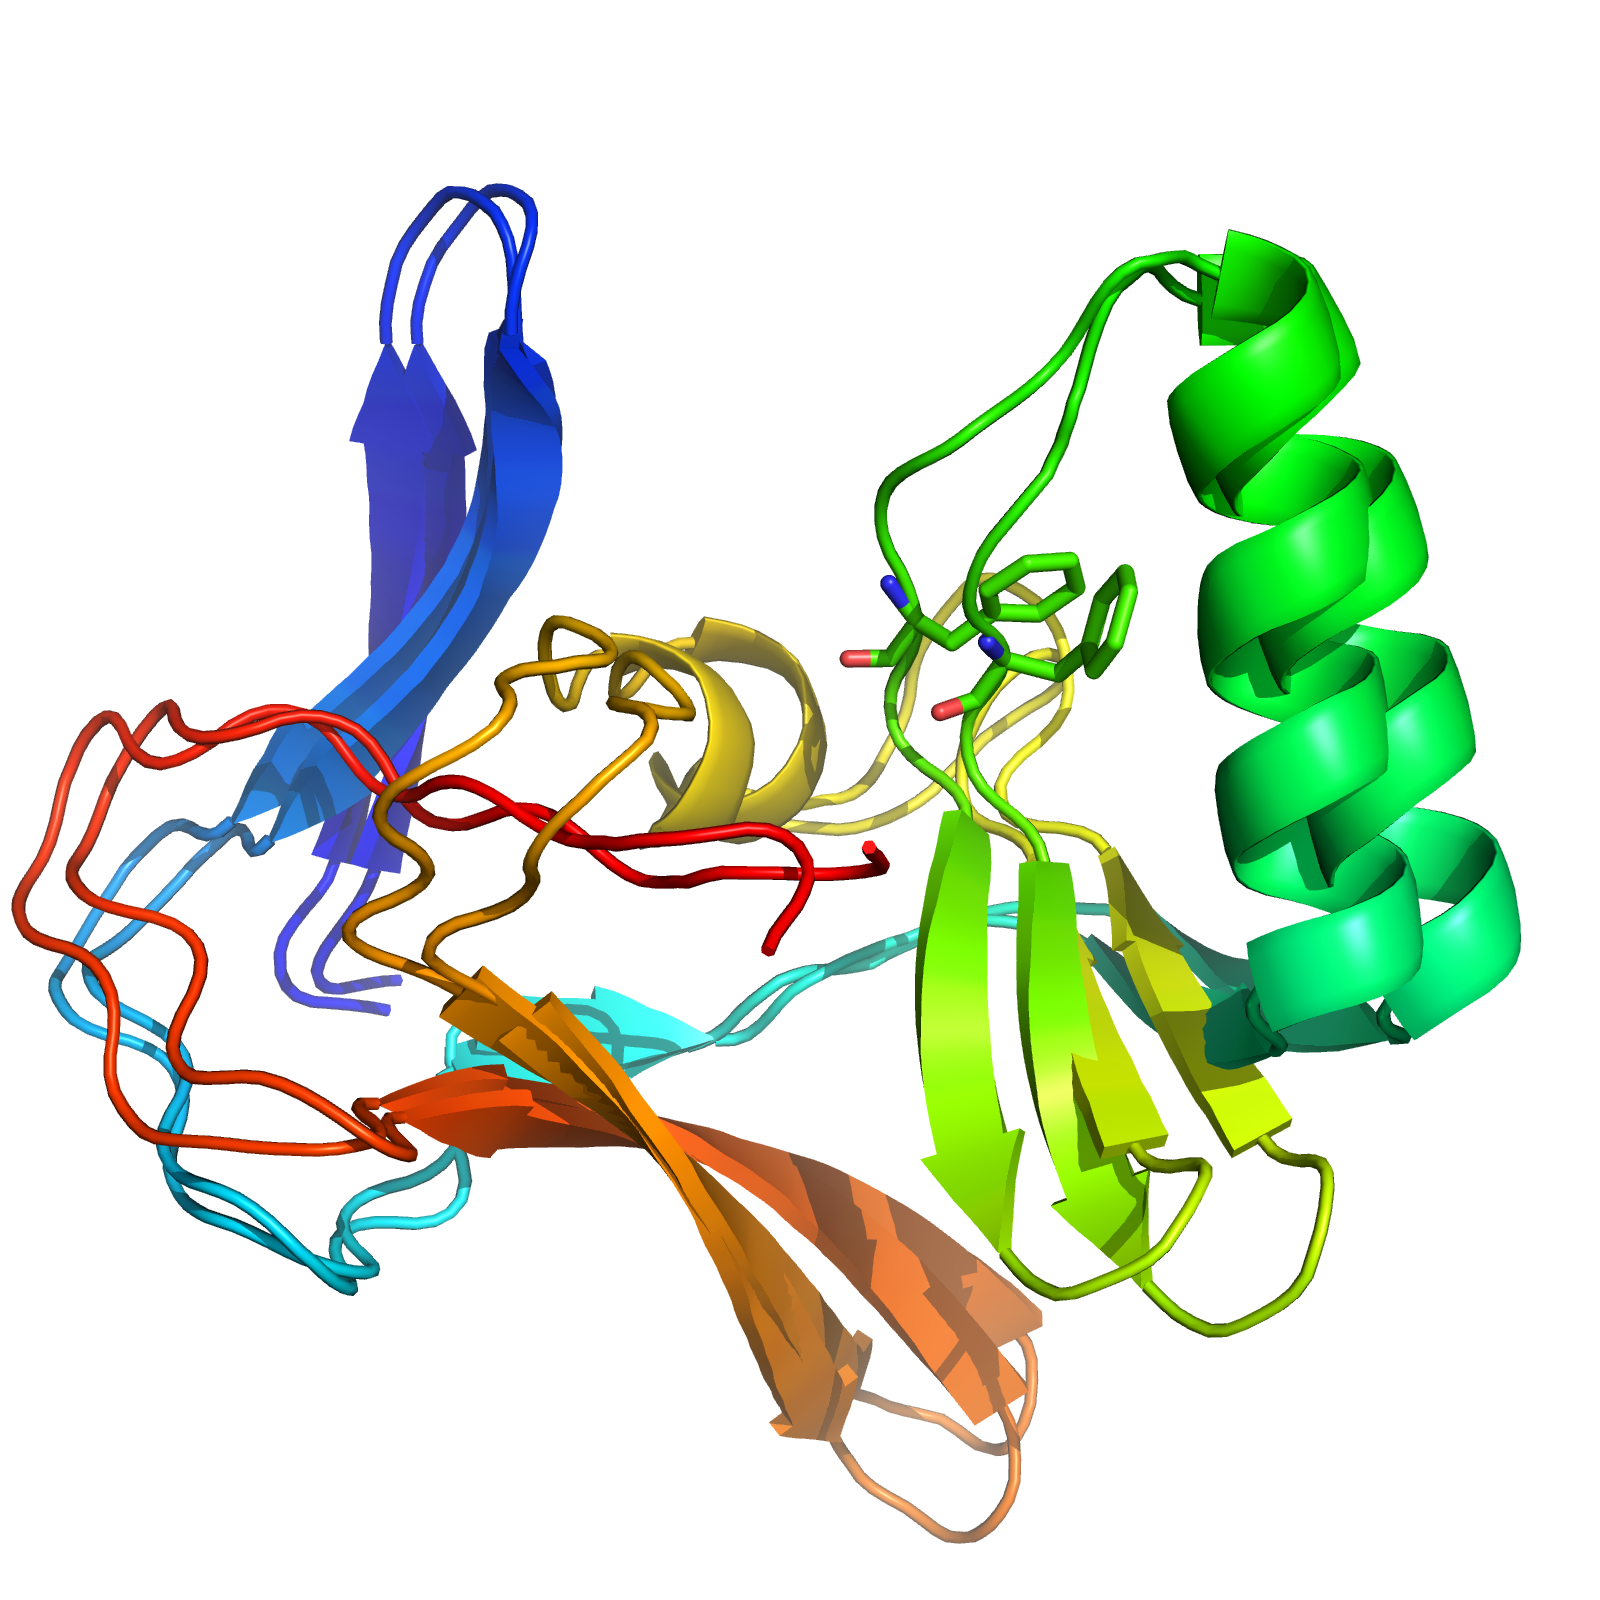
\includegraphics[width=5.0cm]{figures/NSD2_pdb.png}
}

\caption{
(a, b, c).  Conformational landscapes---projections onto the two slowest coordinates---show multiple conformational states observed in simulations at the ~$10 \mu s$ timescale.  (d, e, f). Structural comparison of the two dominant states observed in simulation (rainbow) indicate conformational heterogeneity near the known SAM / sinefungin binding site---particularly in the packing of nearby aromatic side chains.  Ligand-bound crystal structures (pink, cyan) show similar conformational states.  Panels (a, d), (b, e), and (c, f) correspond to the SETD2, NSD1, and NSD2 systems, respectively.  SETD2 bound to SAH (d: cyan) adopts a TYR-up orientation (PDB:4H12), while SETD2 bound to sinefungin (d: pink) adopts a TYR-down orientation (PDB:4HMU).  NSD1 bound to SAM (e: pink) adopts a PHE-up conformation (PDB: 3OOI).  In all three systems, simulations suggest the presence of both conformations in solution, suggesting that predictive models of binding affinity and selectivity will require careful accounting for the conformational preferences of the unbound protein.  In particular, our models predict similar conformational states in NSD2, for which there is currently no crystal structure.
}
\label{figure:MSM}
\end{figure}


\end{document}
